\subsection{\forlnameref Diagrama conceptual}
\label{sec:conceptualModel}

\begin{shaded}
Se facilita un ejemplo para ilustrar la inclusión de figuras en \LaTeX.
\end{shaded}

\begin{figure}[H]
\centering
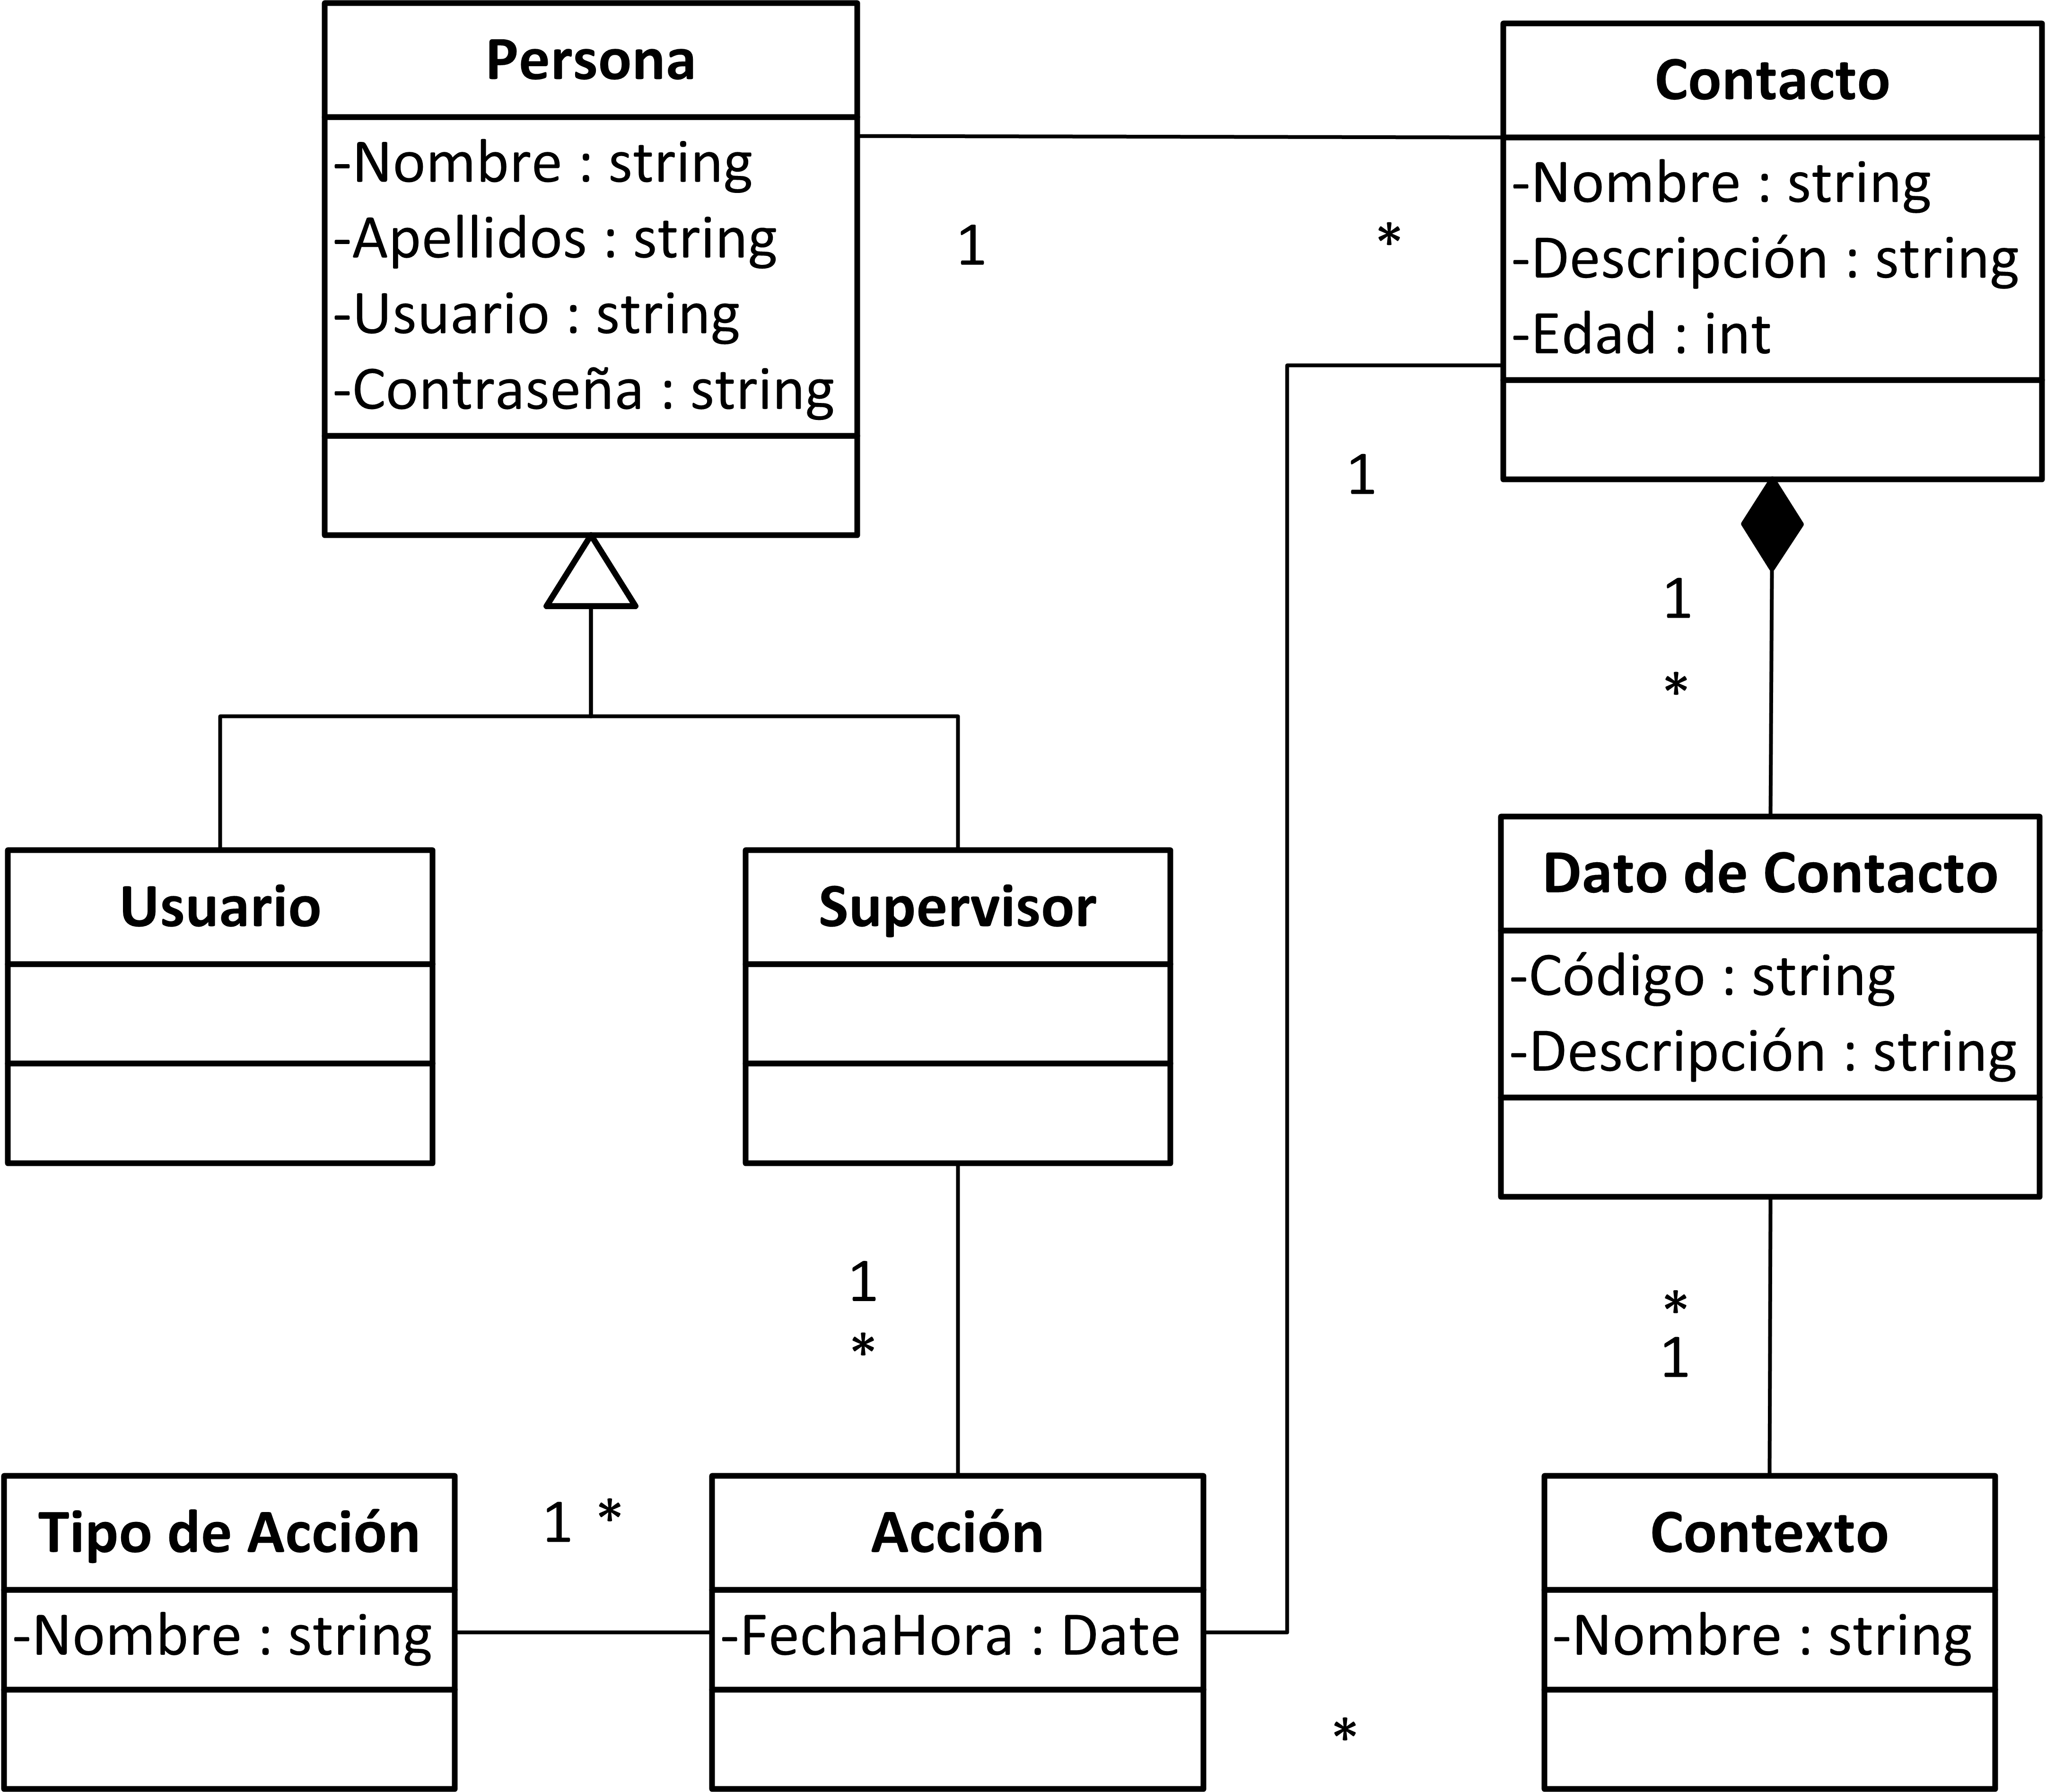
\includegraphics[scale=1]{mco.png}
\caption{Diagrama conceptual}
\label{fig:mco}
\end{figure}

\begin{shaded}
El diagrama conceptual atañe exclusivamente a los requisitos de información, no a los requisitos funcionales. La idea general es ``si no se almacena en el sistema, no existe en el diagrama conceptual''. Todas las entidades y atributos de los requisitos de información deben aparecer en el diagrama conceptual, aunque en éste se permiten estrategias como la generalización o las entidades de relación; es decir, es posible que en el diagrama conceptual aparezca más información que en los requisitos de información, pero no a la inversa.\\

Además de lo indicado, como criterios generales se deben tener en cuenta los siguientes:
\begin{itemize}
    \item Las líneas no expresan acciones, sino relaciones.
    \item Las relaciones con otras entidades no se incluyen como atributos en este modelo (posteriormente sí es frecuente), sino que se indica mediante relación.
    \item Los extremos de las relaciones deben ser cualificados (es decir, tener nombre) si y sólo sí el nombre de dicha cualificación difiere del nombre de la entidad. De otro modo, no sólo no es necesario, sino que resulta contraproducente, al incluir en la vista elementos redundantes. Un ejemplo de cualificación necesaria es cuando una entidad tiene más de una relación con otra entidad.
    \item De igual manera, la propia relación será cualificada cuando no sea evidente (es decir, casos diferentes de ``tiene'', ``contiene'', ``tipifica'', etcétera)..
    \item La composición se emplea cuando un elemento ``se construye'' a partir de otro.
    \item Debe confiarse en la generalización siempre que sea posible.
    \item Hay que perseguir una estética elegante y legible del modelo, si bien en los diagramas grandes puede resultar más complicado.
    \item Si no cabe en vertical, se debe rotar la imagen usando \code{\textbackslash begin\{landscape\}} (del paquete \code{lscape}) en vez de \code{\textbackslash begin\{figure\}[H]}.
\end{itemize}

\end{shaded}